% A description of the software tools that we used.
\section{Software Tools}
In order to meet the objectives that were set at the beginning of the project, we used a wide variety of software tools.
These software tools include database management systems, web frameworks, web page design software, many visualization tools, as well as pieces of software that we have written ourselves.
In the following paragraphs, the various software tools used and their properties will be illustrated.

\subsection{MySQL}
We used the MySQL relational database management system (RDMS) because of three main reasons.
The first reason is that MySQL is an opensource project.
Its source code is licenced under the GNU General Public Licence and therefore this gives us the right to download MySQL and use it free of charge.
Moreover, MySQL is probably the most popular database management system for web applications and several high traffic websites (e.g. Wikipedia, Nokia, Google, Amazon.com and many others) use MySQL in order to store and retrieve data.
Finally, MySQL provides a lot of command line and GUI tools for easy administration and coding.

\subsection{Python}
We chose to use the Python programming language for the development of the KiPhoDB web site because of the reasons presented bellow:
\begin{itemize}
\item Python is a powerful and widely used language, well suited for rapid development. It is pretty easy to pick up by people that do not have prior experience in computer programming, which enables them to learn the basics of this language and contribute to the development of the project in a relatively short period of time.

\item Compared to other programming languages, such as C++ and Java, Python is far less verbose. It is certainly more high-level than C++ and it takes care of memory management. Moreover, it does type checking at runtime rather than at compile time, which means that there is no need to declare types explicitly. Both C++ and Java do not offer this functionality.

\item Python is truly object-oriented (even functions are objects) and it provides a very neat way of declaring and passing function arguments, making functions much more generic than in the aforementionned programming languages.

\item Python excels at parsing (BeautifulSoup, re module for regular expressions) and HTTP access (httplib, urllib).

\item Compared to other scripting languages such as Perl and Ruby, Python is also far more approachable and syntactically more aesthetic. Perl is weakly typed which can a be a source of confusement for various reasons. Ruby would be an interesting alternative but it is unfortunately not widely used or well supported.

\item Choosing Python  allowed us to make use of the brilliant Django-Python framework for rapid database and web site development.

\item One other useful feature of Python is the BioPython library, which provides many tools for automatic data extraction from numerous biological databases (UniProt, PubMed, and many more). Unfortunately, there were a lot of cases when BioPython did not have an appropriate interface for the specific databases we wished to use. In these cases we had to create our own custom interfaces and parsers, which was not a very difficult task due to the fact that Python is particulary well suited for these sort of jobs.
\end{itemize}

Based on the above discussion, we believe that Python was the ideal programming language for the development of the project.

\subsection{Django-Python}
Django is an open source framework for creating web applications.
It is written in python and its source code is released under the BSD license, which gives us the right to download and use Django free of charge.
Django's primary target is to ease the creation of database-driven websites.
It can cooperate flawlessly with MySQL databases and offers an automatically generated administration interface, which allows users to log in and
change entries in the database.
For the aforementioned reasons, we chose to develop KiPhoDB using this framework.
In more detail, we have set up a server using Linux, Apache, MySQL and SSH, which enables each team member to log in and work on the project.
Finally, this server acts also as an experimental server which has helped us to experiment with python and Django in order to accomplish our goals.

\subsection{Dreamweaver}
In order to design the final website, we used the web development application "Dreamweaver".
Dreamweaver is a software product from Adobe and it supports a great variety of web technologies, such as HTML, CSS, JavaScript, ASP and many more.
Nevertheless, only the first two of these technologies were used for the implementation of the main website of KiPhoDB.

\subsection{PhyloWidget}
PhyloWidget is a web-based tool written in Java that enables users to visualize and manipulate phylogenetic tree data \cite{PhyloWidget}.
Its source code is released under the GNU General Public Licence, which gives us the right to use this application free of charge.
We chose to use PhyloWidget and not one of the mainstream phylogenetic visualization and manipulation software tools (e.g. Phylip, PAUP, Mesquite, TreeView) because all these tools are ill-suited for integration with databases and online use.
On the contrary, PhyloWidget offers online tree visualization capabilities, it integrates well with the web environment and it is very easy to configure and use.

\begin{figure}[htp]
\centering
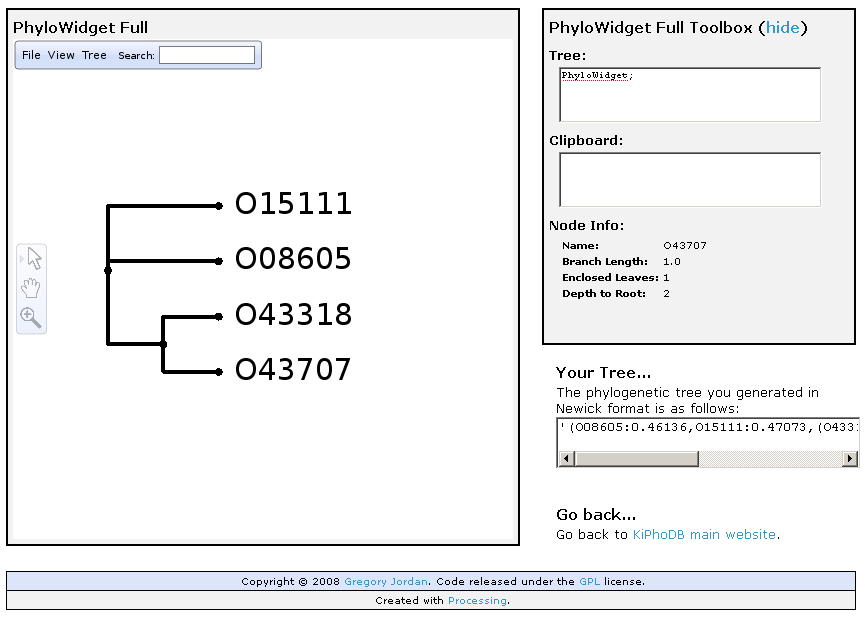
\includegraphics[scale=0.4]{pictures/phylowidget.png}
\caption{The PhyloWidget tool within KiPhoDB's website.}
\label{PhyloWidget}
\end{figure}

In more detail, PhyloWidget offers a simple and powerful user interface that allows users to navigate and manipulate phylogenetic trees by zooming in certain areas, changing the topology of the tree, calculating the distance between certain nodes, copying and pasting subtrees, rerooting the tree and editing the node label or branch length.
When the user clicks on any node, a contextual menu appears that enables users to execute any one of the aforementioned actions.
Moreover, the web interface offers two text fields that are constantly updated and contain the Newick representation of the tree and the clipboard contents.
This feature allows users to easily copy and paste tree string representations from other sources and programs.
Finally, PhyloWidget is able to parse trees in many formats, such as Newick, NHX and Nexus, and it can output trees as images (JPEG and PNG) or PDF files.

One other reason that led us to choose PhyloWidget was its speed and responsiveness even when the program had to visualize a relatively large tree.
For example, a tree with 3000 nodes can be displayed at 30 frames per second, allowing the user to easily navigate through it \cite{PhyloWidget}.
PhyloWidget is the ideal applet for online tree visualization because it is written in Java and therefore it is very fast and efficient and it can be easily and seamlessly integrated in the KiPhoDB web site.

% Development Server
\section{Development Server}
One of the primary tasks that we had to accomplish was to find a development server in order to set up our web site.
This task was very important because we wanted to have a unique place where our web site and database would be stored, instead of having multiple copies of it in each group member's personal computer.
If we had chosen to have multiple copies of the website, these copies would soon get out of sync and it would be very difficult in practice and time consuming to reconcile all the differences and produce a final output.
On the contrary, setting up a development server offers the possibility of using a version control system, which enables each developer to download the changes that other developers have made, make his/her own contribution to the code and finally commit the new changes to the server.

In order to create a development server, we had to choose one out of the following two options.
The first option was to contact the Bioinformatics Support Service of the Bioinformatics Centre or the Computing Department and ask them to set up a development server for us.
Unfortunately, this means that we probably would have to wait many days or even weeks before we could get the development server and start using it.
Of course this is a serious disadvantage, because the project had a very tight deadline and the time that we had to develop, test and debug it was limited.
Therefore we could not waste any valuable time waiting for the construction of the development server from a third party.

One other crucial disadvantage of the aforementioned option is that we would not have any control over the server itself and the software that was installed in it.
This means that we would have to contact the administrators of the server whenever we wanted to use an additional Python library or another program and ask them to download and install it on the server.
Of course, such a procedure would introduce even more delays and waste of precious time.
Moreover, the administrators would be very hesitant to install new software, because they would be concerned about its compatibility and the security issues related to it.
Finally, we would have no guarantee concerning the uptime of the server.

The second option was to use the knowledge, skills and expertise of the group members in order to set up a development server of our own.
We chose this option because it enabled us to avoid all previously mentioned negative aspects and save valuable time.
In addition to that, using a self-made development server allowed us to have ultimate control over the hardware, software, compatibility issues and security issues that the creation of a server involves.
The hardware and software components shown in Figure \ref{logos} and listed below were utilized in order to create our development server:

\begin{figure}[htp]
\centering

\includegraphics[scale=0.6]{pictures/logos.png}
\caption{Software components of the development server.}
\label{logos}
\end{figure}

\begin{itemize}
\item \textbf{Hardware} \\
The computer that we used to set up the server was Christos' laptop with the following hardware characteristics: 1248 MB RAM, 3.06 GHz Mobile Intel Pentium IV processor and 250GB HDD.
The laptop was also connected to the internet through a home router and a high-throughput connection.
Therefore we had to make all appropriate changes to the router in order to allow incoming traffic to certain ports and filter all other malicious internet packets.

\item \textbf{Operating System} \\
We chose to use Arch Linux (Kernel version 2.6.27) instead of Windows XP or Vista because Linux is a much more stable and reliable operating system in comparison to Windows.
Moreover, Arch Linux is a very flexible Linux rolling distribution, which means that it is not under a versioning system and the user can install cutting edge software at any given time without worrying about having an outdated version of the system.
Finally, a user account was created for each member, which could be mainly used for programming purposes and for uploading all necessary files that allowed the server to operate flawlessly.

\item \textbf{Database Management System} \\
As it was mentioned in previous sections, MySQL was the database management system that we chose for the development of KiPhoDB.
The latest version of MySQL was installed on the server for this purpose: Version 14.12, Distribution 5.0.75.

\item \textbf{Django} \\
Django version 1.0.2 was also set up on the server.
Moreover, we also had to install numerous python libraries that proved to be very useful for data mining, string matching, xml and html parsing, timing and many more (BeautifulSoup, BioPython, xlrd, etc).

\item \textbf{HTTP Web Server} \\
Apache is a powerful web server that has been chosen to host KiPhoDB.
The version used was 2.2.11 and we also installed various modules that enabled Apache to dynamically execute python scripts and display the results as html files (mod\_python 3.3.1, Python 2.6, mod\_ssl 2.2.11, etc).

\item \textbf{SSH} \\
The SSH protocol is widely used for establishing a connection to a remote server and executing commands.
We installed SSH to the server, so that the users could connect to it and either submit their work or execute various python scripts for updating the database.

\item \textbf{Version Control} \\
The version control system we used is called SubVersion (SVN) and we installed the latest version of it, namely 1.6.0.
This system proved to be very useful, because it provided a unified resource for the source code of KiPhoDB.
Therefore each one of us was able to commit his/her work on the server so that all other group members could view, test, debug and build upon it.
By using SVN we managed to avoid having multiple versions of the source code in our computers, which of course would make it very difficult to combine them at the end and form the final web site.

\item \textbf{URL} \\
Of course a proper web server should have its own URL, which can be used by the web site's users in order to easily access it.
The problem we had to face in this case was that the internet connection of the development server did not offer a static IP.
On the contrary, each time the connection was lost or the router was restarted, a new IP address was assigned to the computer.
Therefore we had to use dynamic DNS services, such as the ones offered free of charge from the company DynDNS.org, in order to book the following url: dbproject.dyndns.org.
\end{itemize}

In conclusion, the creation of our own MySQL and web server has proven to be a very wise decision, because of the reasons that were mentioned previously in this section.
Furthermore, until now the development server has worked flawlessly and it has provided us with all necessary resources to work on the development, testing and debugging of KiPhoDB.
At the time of writing, the server has been up and running for 34 days, 5 hours and 28 seconds, having an overall uptime of more than 99\%.
Nevertheless, once KiPhoDB is complete, it should move to a proper production server, which will provide additional security features and functionalities.
Moreover, the production server will have greater processing power and more memory, so that it can process simultaneous requests of many users.

% The database schema.
\section{Database Schema}

Creating the KiPhoDB database schema was one of the most difficult parts of this project.
This is because the database schema should reflect as accurately as possible the different biological structures and processes found in nature.
Additionally, it should contain all necessary tables and fields that would provide adequate storage space for all available biological data.
One other aspect of the Database Schema that made its creation a challenging task is that it should be normalized and strictly follow at least the third normal form.
We believe that at the end we managed to create a very robust but yet flexible database schema that provides users with all useful information about kinases, phosphatases and their substrates.
At this point we would like to acknowledge the support of Prof. Michael Stumpf and Dr. Frances Turner, who helped us significantly in the process of creating the database schema for KiPhoDB.

\begin{figure}[htp]
\centering
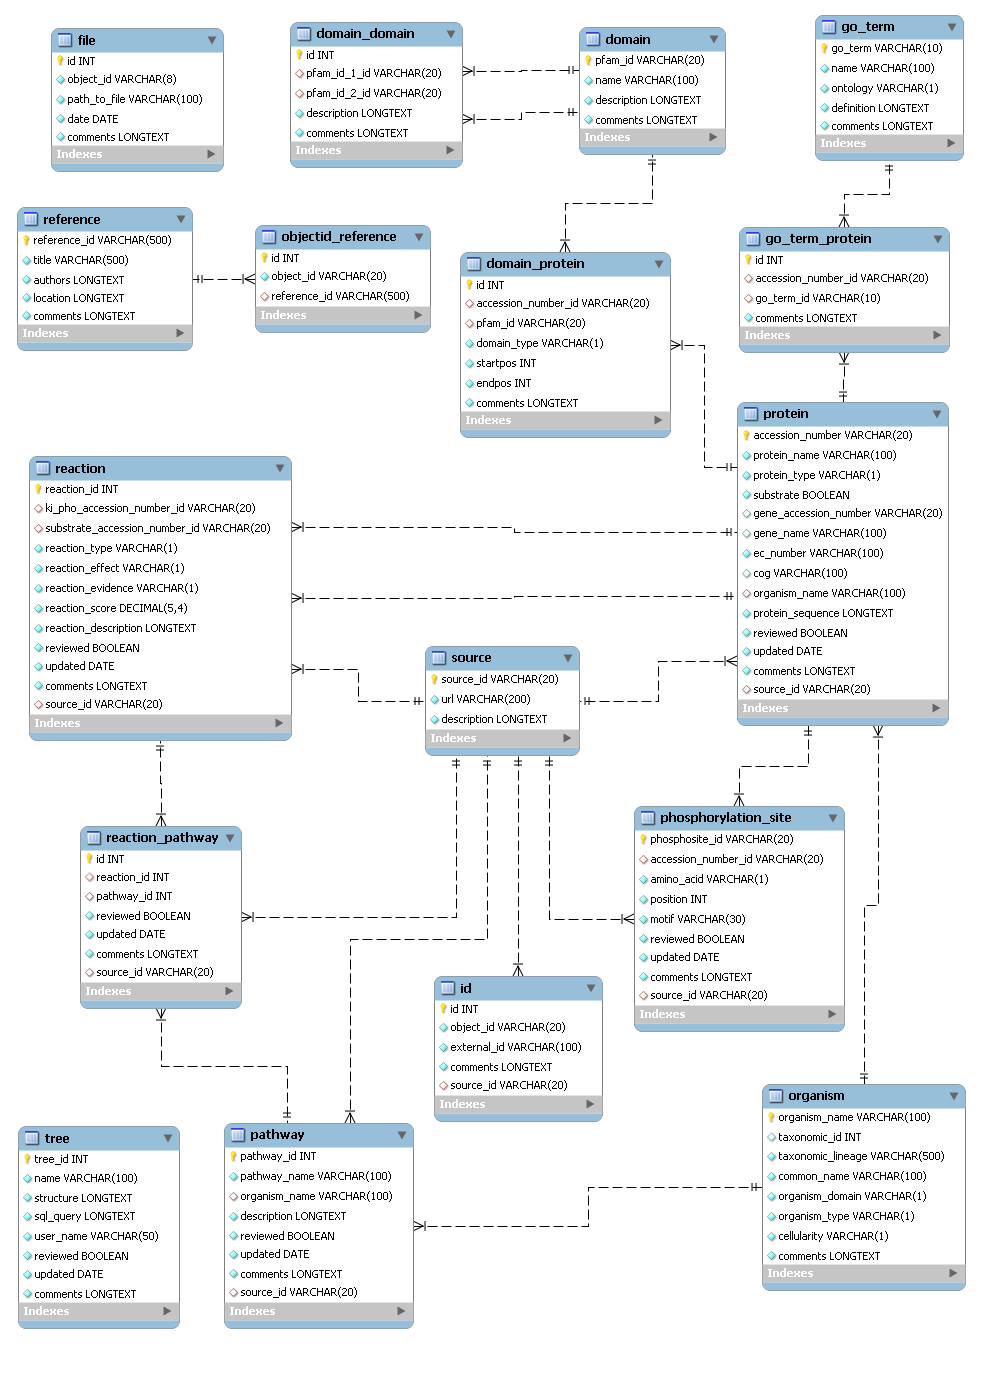
\includegraphics[scale=0.43]{pictures/DatabaseSchema.png}
\caption{The Entity Relationship (E/R) diagram of the KiPhoDB database.}
\label{DatabaseSchema}
\end{figure}

It was previously mentioned that, in general, a database schema should be normalized and follow at least the third normal form.
The reason for this is that non normalized databases have many significant disadvantages compared to properly normalized databases.
Therefore active steps must be taken in order to ensure that the database we create is properly normalized.
Perhaps the most significant property of normalization is that it makes a database much more flexible and considerably less prone to errors.
Moreover, it makes the data model more informative to the users, successfully avoids modification anomalies and minimizes the redesign efforts in cases when we want to expand the database.
Based on the above discussion, we worked hard to produce a normalized database schema and we believe that at the end our efforts were successful.

The database schema of KiPhoDB is illustrated in Figure \ref{DatabaseSchema}.
As it is shown in this figure, KiPhoDB contains seventeen tables in total.
The main table of our database is the \textsl{Protein} table, where all kinases, phosphatases and substrates are stored.
Since all these three molecules are actually proteins, it is not advisable to create three different tables that will consist of exactly the same fields.
Instead, it is much better to have one table where all this information will be stored and easily retrieved afterwards.
All interactions between the proteins of this table are stored in another table named \textsl{Reaction}.
As the name implies, the Reaction table stores information about reactions between pairs of proteins and various details about each reaction.
These can be both phosphorylation and dephosphorylation reactions which can lead either to the activation or deactivation of the corresponding substrate.
Furthermore, each reaction is considered to be part of a specific pathway and therefore a foreign key relationship exists between the Reaction and the \textsl{Pathway} tables.
Needless to say that the Pathway table includes further information about pathways in different species.

For every protein in the Protein table, its phosphorylation sites, domains and GO terms are stored in different tables.
This information is very important because a researcher needs to know the exact position in the amino acid sequence where the phosphorylation takes place, the various domains that a kinase/phosphatase/substrate contains and its GO term annotation.
All these data are stored in tables \textsl{Phosphorylation Site}, \textsl{Domain} and \textsl{GO term}, whose contents are self explanatory.
These three tables have strong interconnections with the Protein table and therefore the appropriate foreign key relationships have been defined in the database schema.
The connection between the Protein table and the Domain and GO term tables is a many - to - many relationship and therefore additional tables have been created that implement these relationships.
In this way our database is normalized and has all the advantages presented presiously in this section.
On the contrary, the connection between the Protein table and the Phosphorylation Site table is an one - to - one relationship and therefore the creation of a simple foreign key on the Phosphorylation site table has been sufficient.

In addition to the tables mentioned above, we have also created some tables that extend the functionality of our database.
These tables are named \textsl{Reference}, \textsl{File}, \textsl{Tree}, \textsl{Organism} and \textsl{ID}, and store references, files, phylogenetic trees, organisms and external IDs respectively.
Including this kind of information in our database is vital because in this way our database is enriched significantly and it also becomes more comprehensive.

%Data Input
\section{Data Input}
In order to populate the KiPhoDB database we had to utilize a great variety of biological data sources.
All available data sources had to be thoroughly investigated, so that we could estimate the quality and quantity of data they offered.
At the end we reviewed the available information about each source and decided to use only those that provided easily retrievable data of high quality.
These sources and some of their main characteristics are summarized in the third chapter of this report.
Here we will provide the reader with a brief description of the data extraction techniques that we used in order to retrieve data from those sources and successfully insert them in our database.

The most common way to extract data from a resource is to write a parser.
The main aim of the parser is to read the data from a database, a flat file or the internet and convert these data into the appropriate format so that they can subsequently be easily inserted in the database.
In essence, a parser is a tool that is used to change the data container, but leave the data themselves intact.
Of course, the data from various sources where in different formats and therefore we could not use a single generic parser.
On the contrary, we had to create one or more parsers for each data source.
In the following, an overview of the various data formats that we had to deal with and the techniques that we used to extract interesting data are presented.

\begin{itemize}
\item \textbf{BioPAX} \\
BioPAX stands for Biological Pathway Exchange and it is an emerging format for representing molecular interactions, gene regulation networks and signalling pathways.
Comparing to other established formats, BioPAX offers a better representation of various physical states of the protein and contains more information about the protein itself (amino acid sequence, name, external references and other features).
Furthermore it offers the ability to accurately represent gene regulation networks and gene expression regulators, such as transcription factors, microRNA, etc.
Finally, the BioPAX format is able to include information about degradation substrates in various pathways and various genetic interactions which are important for mapping pathways.
We encountered this format while manipulating the data from NetPath, a curated database for immune and cancer signalling pathways created by HPRD (Human Protein Reference Database).

\item \textbf{HTML/XML} \\
The KiPhoDB database contains a lot of information from UniProt, which offers its data in HTML or XML format.
These two formats are some of the simplest formats available and we had to create parsers that would extract the desired information and input it into our database.
Fortunately there are a lot of libraries for the Python programming language that enable programmers to easily parse such files.
One such library is DOM, which stands for Document Object Model and it provides us with all necessary methods for accessing and manipulating XML documents.
DOM presents a tree view of the document under examination, with a root node, many child nodes and the leaves.
In every case, the root node is used to read, write and modify each one of the child nodes.
Our parser scripts made extensive use of the minidom Python library, which is a lightweight implementation of the DOM interface.
Its main characteristics is its simplicity and flexibility compared to the full DOM library, which enabled us to quickly and easily learn how to use it and start writing the parsers without wasting any time.

One other library that we used for parsing HTML files is called BeautifulSoup.
This is a very powerful Python library which offered us the ability to search for keywords in HTML documents using the appropriate regular expressions.
Subsequently we were able to extract the required information from any HTML file and insert it into the appropriate table of our database.
BeautifulSoup is ideal for screen scraping and it offers a wide variety of powerful data extraction features, which made it the ideal library for our purposes.
However, the main drawback of BeautifulSoup is that it is much slower than other available HTML parsers, but overall it has many positive characteristics and this is the reason why we chose to use it.
Its main use was to extract pathway data and subsequently update the appropriate tables in the database.

\item \textbf{XLS} \\
Some data sources, for example PHOSIDA, offered their data in xls format.
This format is used by Excel\textsuperscript{\texttrademark}, a very popular popular spreadsheet product from Microsoft\textsuperscript{\texttrademark}.
In order to parse this kind of files we had to use the xlrd Python library, which allows developers to read, write and extract information from files having the xls format.
The main strength of this library is that it is written purely in Python and it can manage unicode encoded xls files.
Moreover it offered us the possibility to read each sheet of the file separately and thus manage to get the required information quickly and easily.

\item \textbf{TSV/CSV} \\
PhosphoELM and a few other data resources gave us flat files that contained information in TSV (Tab Separated Values) or CSV (Comma Separated Values) format.
As the name implies, these files contained fields that were separated either by tabs or by commas.
This kind of files can be easily imported in the database using Python's build-in split function, which returns a list with all the contents for each line.
Therefore flat files in TSV or CSV format were not a particular problem for us and we were able to create all necessary parsers for them.

\end{itemize}

At this point it is useful to note that we also made extensive use of the Biopython library for Bioinformaticians.
This library provides a wide variety of tools and modules that enable every Python programmer to acquire biological information from a variety of online sources.
One of its main functionalities is that it can automatically connect to NCBI, EBI, UniProt and many more online resources of data, download information and make it available to the programmer.
In addition to that, it also provides easy to use interfaces to common bioinformatics programs, such as NCBI Blast.
It can perform sequence translation, transcription and weight calculations.
For the purpose of this project we only used a subset of the BioPython features in order to automatically retrieve protein information from UniProt and update KiPhoDB's entries accordingly.
Finally, we also used BioPython to fetch information and details from NCBI about each PubMed entry in our database.

%WebSite
\section{Web Site}
KiPhoDB's central web site is presented in Figure \ref{website}.
As shown in the picture, the web site's design is simple but at the same time flexible and powerful.
Its main purpose is to provide users with all necessary software tools in order to enable them to easily and effectively exploit all data contained in our database.
Moreover it also includes a lot of information about the database itself, its contents and legal information about its usage.
Finally, the web site aims to provide a pleasant and productive environment which users can use in order to find answers to their research questions.

\begin{figure}[htp]
\centering
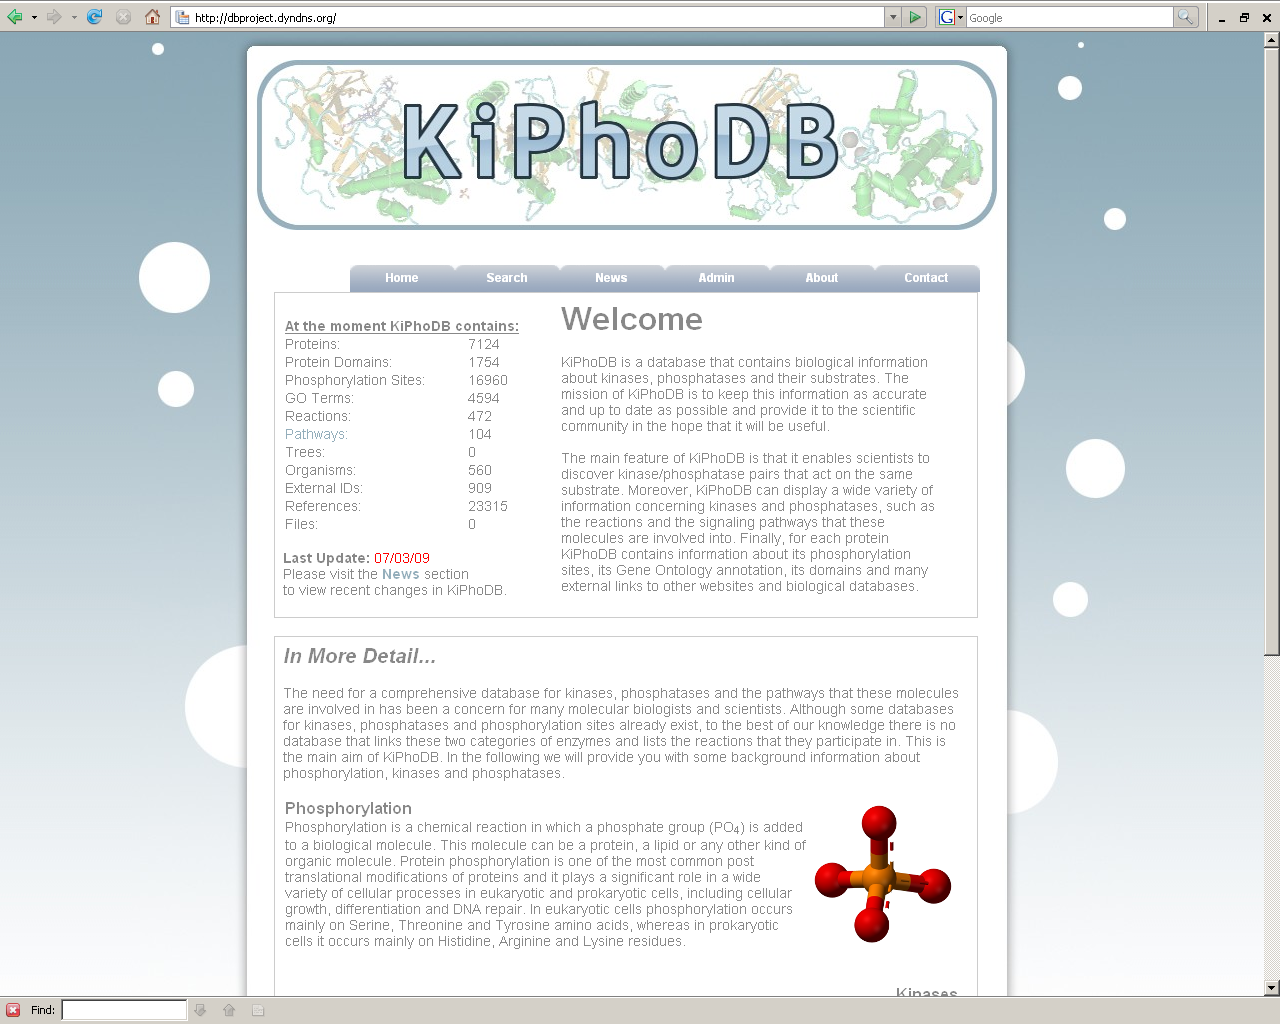
\includegraphics[scale=0.35]{pictures/website.png}
\caption{The KiPhoDB website.}
\label{website}
\end{figure}

\begin{figure}[htp]
\centering

\includegraphics[scale=0.6]{pictures/license.png}
\caption{KiPhoDB's license}
\label{license}
\end{figure}

Table \ref{table:WebSiteStructure} further illustrates the internal structure of the web site and the pages that it consists of.
The table itself is pretty explanatory and it provides the URL of each page, its title and a brief description of its contents.
Therefore in the following paragraphs we will only focus to some aspects of the website that deserve further explanation.

\begin{table}[h]
\vspace{1cm}
\footnotesize
\begin{center}
\begin{tabular}{ | l | c | l | }
\hline
\textbf{URL} & \textbf{Name} & \textbf{Description} \\
\hline
\hline
/index.html & Home & A welcome page which provides some statistics about the contents \\
& & of KiPhoDB and theoretical information about kinases, phosphatases \\
& & and substrates. \\
\hline
/search.html & Search & This page can be used to access the various database mining \\
& & tools provided by KiPhoDB. These tools enable each user to \\
& & extract information from the database or create phylogenetic \\
& & trees based on KiPhoDB's data. \\
\hline
/news.html & News & All news, latest updates and releases concerning the KiPhoDB \\
& & database or the web site are made public in this page. \\
\hline
/admin/ & Administration & The administration interface of KiPhoDB. The user name and \\
& & password is required in order for a user to have access \\
& & to this part of the web site. \\
\hline
/about.html & About & This page provides information about KiPhoDB, its creators and \\
& & the technologies used. Moreover, it provides a link that \\
& & enables users to download the database and install it locally \\
& & on their computers. \\
\hline
/contact.html & Contact & Legal information and contact details are provided in this page.\\
& & In order to leave a comment, users can either send an email \\
& & to the administrators or fill in and submit an online form. \\
\hline
/results.html & Results & When a user performs a simple search, all results are analytically \\
& & displayed on this page. \\
\hline
\end{tabular}
\end{center}
\normalsize
\caption{The structure of KiPhoDB's website.}
\label{table:WebSiteStructure}
\vspace{1cm}
\end{table}

One of the aspects that should be mentioned and analyzed concerns the legal status of KiPhoDB.
We have chosen to release KiPhoDB under the Creative Commons Attribution + Noncommercial + NoDerivs license, a graphical representation of which is shown in Figure \ref{license}.
This means that each user is free to copy, distribute and display the information stored into the KiPhoDB database and its public website under all legislations, provided that he/she will give credit to the creators of KiPhoDB.
Nevertheless, users do not have the right to use the contents of KiPhoDB for commercial purposes or distribute a modified version of it.
A user can do this only if he/she contacts the developers of KiPhoDB and gets a written permission to do so.
On one hand, this license gives users all necessary permissions to use KiPhoDB free of charge and without violating any copyright laws, but on the other hand it restricts their ability to use KiPhoDB for commercial purposes or distribute a modified version without our prior written permission.
These two characteristics of this license make it ideal for the purposes of KiPhoDB and therefore we decided to adopt it.
Of course, similar licenses have commonly been used in a wide variety of Bioinformatics websites and databases.

Every database should ideally ask for user feedback in order to improve the quality of the data that it contains and the services that it offers to the public.
We believe that user feedback is a very powerful tool that will help us improve KiPhoDB's services and data.
Consequently we encourage users to report any errors they find and send us comments, ideas and suggestions.
This can be achieved either by sending an email to KiPhoDB's email address or by completing an online form that we have set up solely for this purpose.
The online form has the following fields: Name, email, URL and Comments.
Once the form is completed and the button ``Post" is pressed, the information is stored into the database itself and the administrators can view it at their own time.

One other characteristic of the website that should be mentioned is that it offers users the ability to download the entire KiPhoDB database and set up a copy of it in their local servers.
This feature can be found in the ``About" page, along with a short description of the database itself, the software technologies that have been used to create it and short biographies of the people behind this project.
KiPhoDB data are offered in a single \verb+.sql+ file which was created directly from the MySQL database using the program \emph{mysqldump}.
The size of this file can be tens of Megabytes and this is the reason why we have to use compression in order to make it smaller.
Once the file has been successfully downloaded from KiPhoDB's web server and properly extracted, it is pretty straight-forward to import it in the local MySQL server and use it.
This characteristic of the website is very important because it allows users to work on their own local copy of KiPhoDB instead of sending their queries to KiPhoDB's server and thus increasing its load.
Nevertheless, it should be noted that the sql file has to be updated regularly so that it can reflect all recent changes made to KiPhoDB.

The administration interface can be accessed through the ``Admin" button and it is one of the most important parts of the website.
Its main function is to allow authorised users to view, modify and delete the contents of our database, primarily for maintenance purposes.
Public users are not allowed to perform such kind of operations, but only to view the contents of the database and combine the information stored in different tables in order to produce answers to their queries.
On the contrary, a small number of individuals will have administrative access, which means that they will receive a certain user name and password combination in order to be able to use the administration interface.
These individuals will be charged with the duty to routinely maintain the contents of the database, read the feedback provided by KiPhoDB users and take all appropriate steps to improve the data and the services provided.
As part of the routine maintenance, which should be performed on a regular basis, we have created automated Python scripts that can update certain database tables in a matter of minutes.
These scripts have been proven to be very useful and they have significantly simplified the task of maintaining the contents of KiPhoDB up-to-date.

%Database search tools.
\section{Database Search Tools}
The ``Search" page of the website hosts all software tools that we created in order to enable every user to search the KiPhoDB database and find all necessary information.
We believe that it is very important for every database to provide users with a plethora of powerful tools that will give them the opportunity to exploit the database in every possible way.
Therefore we created seven distinct software tools, which will be examined in more detail in the following sections.
Each one of these tools has its own strengths and weaknesses and can be used for different purposes.
Additionally, the user can combine two or more of these tools in order to get the information that he is looking for.
In the next sections we will provide the reader with more details about each tool, its main features, strengths and weaknesses.

\subsection{Kinase - Phosphatase Pairs}
\begin{figure}[htp]
\centering
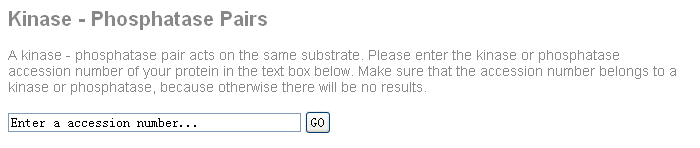
\includegraphics[scale=0.6]{pictures/PairSearchTool.png}
\caption{Search Tool for Finding Kinase-Phosphatase Pairs}
\label{PairSearchTool}
\end{figure}
A kinase -- phosphatase pair is a combination of a protein kinase and a protein phosphatase that act on the same substrate.
Finding kinase -- phosphatase pairs is very interesting for biologists and one of the primary objectives of this project.
The Kinase -- Phosphatase Pairs Tool has one purpose: to enable users to identify kinase -- phosphatase pairs based on a given kinase or phosphatase protein molecule.
The user simply has to input the accession number of a protein kinase or protein phosphatase that he/she is interested in.
Subsequently the tool performs a search in the Reaction table of the database and tries to find reactions that involve the given protein.
In this way, all substrates can be positively identified and the corresponding kinase/phosphatase molecules can be found based on the common substrate.
As a result, users will be provided by a list of kinase-phosphatase pairs along with their corresponding reactions.
If the protein that the user has input is neither a kinase or a phosphatase, this tool will not produce any results.

\subsection{Simple Search}
\begin{figure}[htp]
\centering
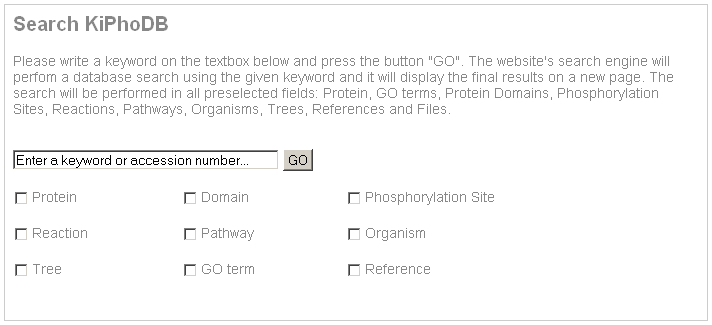
\includegraphics[scale=0.6]{pictures/SimpleSearchTool.png}
\caption{The Simple Search tool.}
\label{simplesearchtool}
\end{figure}
The main purpose of this tool is to enable users to perform simple searches in the database.
It is clearly illustrated in Figure \ref{simplesearchtool} that this tool consists of a text box, where the user can insert one or more keywords, nine checkboxes, where the user can select the tables that will be examined, and one button to initiate the search.
Once the button has been pressed, the server executes a script which searches all preselected tables of the database for the given keyword.
The results of this script are subsequently displayed on a different page.
Of course, it is possible to select more than one check boxes in order to perform a keyword search in more than one table.
This will display all entries in the specific tables that contain this keyword.

For example, if a user wants to find how may pathways in the database are involved in signalling, he/she will check the ``Pathway" check box, write the word ``signalling" into the textbox and initiate a database search by clicking on the ``GO" button.
This will display a new page containing the results of the investigation, namely the pathways that contain the keyword ``signalling".
The results contain among others the Oxidative stress response pathway, the Opioid Signalling pathway and the Integrin signalling pathway.
By clicking on any one of these pathways, the user can view more details about it: the organism that this pathway appears in, a brief description, some comments and the reactions that is is involved in.
By clicking on any of the aforementioned reactions, the user can display more information about the reaction itself and the proteins that take part in it.
For each one of these proteins, the user can also find out which other reactions they participate into, the exact location of the phosphorylation sites in the amino acid sequence and much more information.

The example of the previous paragraph clearly illustrates the fact that the simple search tool provides an easy way to find proteins, domains, phosphorylation sites, pathways, reactions, etc, related to a specific keyword.
Moreover, the interconnections that exist between the various entities of KiPhoDB can help users investigate any potential connections between the objects of their queries and other objects in the database.
This can be very useful when, for example, one is trying to identify which phosphatase dephosphorylates a substrate that was previously phosphorylated by a given kinase and vice versa.
Using the database, one can create a list that contains all substrates that a kinase phosphorylates and then find the corresponding phosphatases by searching the Reaction table for the inverse reactions.

In conclusion, the Simple Search tool is very useful in cases when a user wants to find out if a certain protein, phosphorylation site, pathway, etc, exists in KiPhoDB and what other information the database contains for this object.
Unfortunately, this tool does not support advanced database searches and finding answers to more complex queries by combining more than two database tables.
For this purpose we have developed other more sophisticated tools, which we will describe in the following sections.

\subsection{Advanced Search}
\begin{figure}[hp]
\centering
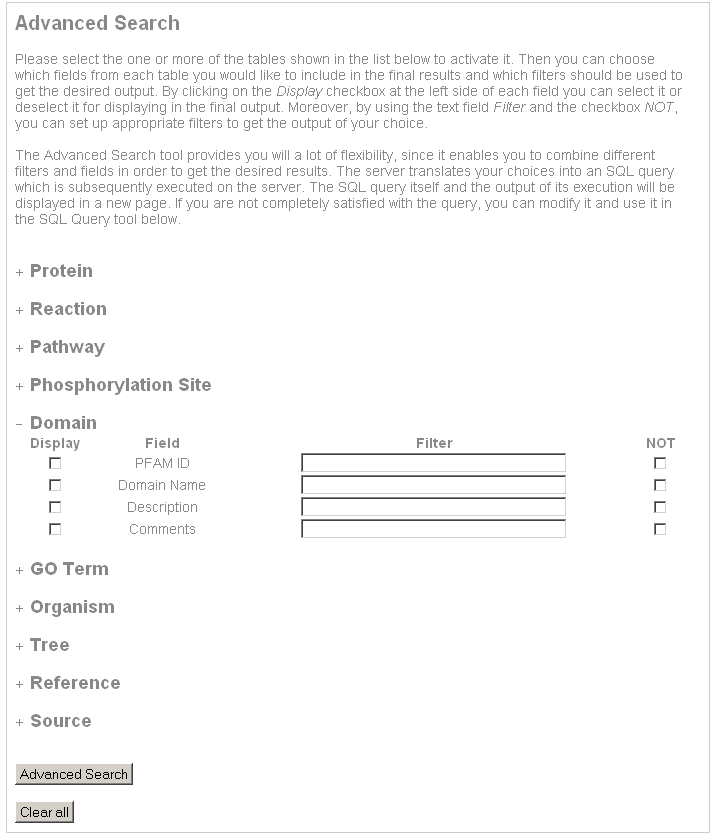
\includegraphics[scale=0.6]{pictures/AdvancedSearchTool.png}
\caption{The Advanced Search Tool.}
\label{advancedsearchtool}
\end{figure}
The Advanced Search Tool extends the functionality of the Simple Search Tool by providing the user with more options and possibilities.
Its main purpose is to provide visual aids to users in order to enable them to easily and quickly construct their own SQL Queries and run them on the MySQL server.
The tool itself consists of an extensive list of all available tables in the database.
Once the user selects one or more of these tables, these tables are activated and an extensive list of each table's fields appears.
As shown in Figure \ref{advancedsearchtool}, this list can be used in order to apply filters and determine the exact output of the query.

At the beginning, the user has to choose which fields from each table should be included in the final results.
This can be achieved by checking the appropriate check boxes under the column ``Display" that correspond to the fields of his/her choice.
Subsequently the user has to define some filters that will restrict the output and display only the necessary information.
If no filters are defined, the Advanced Search tool will display all information available, without applying any filters.
In order to set up a filter, the user has to use the text field under the column ``Filter" and next to the name of the field he/she is interested in.

In this paragraph we will examine a comprehensive example of the procedure mentioned previously.
Let us assume that a user wants to display the accession numbers and names of all proteins that contain the domain with Pfam ID PF10584.
In this case, he/she would have to follow this procedure:
the first step would be to select the display check boxes located next to fields ``Accession Number" and ``Name" of the ``Protein" table.
Then he/she would have to set up a filter on the ``Pfam ID" field of the ``Domain" table by writing ``PF10584" in the appropriate text box.
Finally, after pressing the ``Advanced Search" button at the bottom, the tool will construct an SQL query and display it to the user along with the results.

Overall, the Advanced Search tool provides users with a lot of flexibility, since it enables them to combine different filters and fields in order to get the desired results.
Moreover it is ideally suited to users that do not have any previous experience with SQL, because it automatically constructs the SQL query for them based on their choices.
As mentioned before, the output of this tool consists of both the generated SQL query and the results of running it on the server.
If a user is not completely satisfied by the SQL query that this tool has automatically generated for him/her, then he can modify it and run it again by using the SQL Query tool described in the following section.

\subsection{SQL Query}
\begin{figure}[htp]
\centering
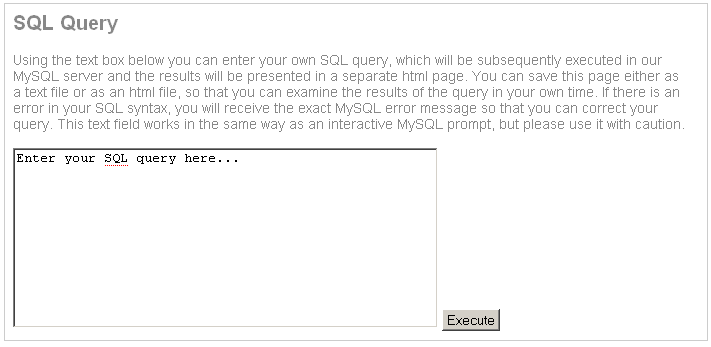
\includegraphics[scale=0.6]{pictures/SQLQueryTool.png}
\caption{The SQL Query Tool.}
\label{sqlquerytool}
\end{figure}
As shown in Figure \ref{sqlquerytool}, the SQL Query Tool consists of a text area where the user can type in SQL commands and a button to execute the query.
Once the user enters an appropriate SQL command and presses the ``Execute" button, the system reads the command and sends it to the KiPhoDB MySQL server for execution.
When the execution of the query has finished, the tool retrieves the results and displays them to the user in a tabular format on a different html page.
Of course, the results can be easily saved as an html or text file by making the appropriate selections on the menu of the browser that is being used.
This feature enables users to further process the results with other external tools in order to get the information they are seeking.

There were many security challenges involved in the creation of this software tool.
It is a fact that giving direct access to a MySQL prompt to the public user is not safe for the server and the database.
Therefore active steps must be taken in order to secure the server and protect it from attacks launched by malicious users.
The most important measure that we took for this purpose was to create a separate MySQL user account that had restricted access to the database.
This account did not have the rights to delete or alter the database in any way and, additionally, it could not view some tables that contained information about the other accounts on the system.
The only actions allowed for this account was to execute SELECT statements only to the tables that contained biological information.
This account was exploited in order to run all user generated scripts, effectively shielding the server from any attempts to alter the contents of the KiPhoDB database.

One other security issue that we had to face was the following:
there are some SQL queries that combine information from multiple tables in order to produce a response.
If the number of tables combined is large, the SQL query takes longer to execute.
Therefore it is not safe for the server to allow users to combine information from various tables, because their query can take too much time to execute and restrict other users from using the server or even render it unresponsive to requests from other individuals.
Although there are a variety of measures that can be employed in order to eliminate this threat, we have chosen not to restrict the users' access to the database in any way.
We want the user to be able to execute advanced queries and combine information for various tables in order to find answers to his/her questions.
If we had chosen to take one or more of the aforementioned measures, this would not be possible.
Therefore, the correct function of this tool is primarily based on the responsibility of the users.
Nevertheless, if we suspect that someone is using this tool for non-authorized purposes, we will take immediate action in order to restore and ensure the well being of the database and the server.

In conclusion, this tool is very helpful for advanced users that need to have unlimited access to the database and execute their own queries.
These queries may combine one or more tables to produce the desired response.
In order for a user to be able to use this tool, adequate knowledge of the internal structure of the database is required.
There are two ways to acquire this kind of knowledge.
The first one is to use specific SQL queries that list the tables of the database and the fields that these tables consist of.
For example queries such as ``SHOW TABLES;" and ``SHOW FIELDS FROM Protein;" can be utilized for this purpose.
The second way is to view an image of the Entity -- Relationship model of the database, which includes all tables, their fields and the foreign and primary keys of the database.
A link to this image is located at the bottom of the Search page, along with some explanatory information about the database itself.

\subsection{Browse Data}
As the name implies, the Browse Data tool enables users to browse the data in our database by displaying the contents of different tables, fields that have the same characteristics and their interconnections.
In order to construct this tool we have exploited the automatically generated Django application named ``DataBrowse".
This application inspects the database model and tables in order to dynamically create a rich and browsable web site that enables users to browse all data inside the KiPhoDB database.
Moreover, it gives users the opportunity to classify data according to certain criteria and find entries that have similar characteristics.

The main drawback of this tool is that the DataBrowse application is relatively new and is current under active development by the Django software team.
It became available after Django version 1.0 and therefore there are a lot of improvements that still need to be implemented by the Django developers in order for DataBrowse to become a better tool that will offer users more functionality and ease-of-use.
Nevertheless, we have decided to include this tool and provide it to the KiPhoDB users.
Although, of course, there is still a lot of room for improvement for DataBrowse, the tool in its present state can still offer some functionality that will help users to browse our data and obtain a general understanding about the contents and structure of our database.
In addition to that, it is particularly useful in cases when a user wants to classify the available data according to specific fields.
Therefore we have taken the decision to include it in the list of available software tools for data analysis.

\subsection{Construct Phylogenetic Trees}
This is one of the most important tools in the data analysis toolbox that KiPhoDB provides its users with.
It enables users to perform multiple sequence alignments of proteins that already exist in the database and construct phylogenetic trees according to the results.
The generated phylogenetic trees can subsequently be used to compare proteins and find groups of proteins that have similar structure and function.
This can offer valuable insight into the evolution of various protein kinases and phosphatases and the evolutionary distance between them.
Moreover, it can help scientists identify orthologous and homologous genes and infer information about the structure and function of novel protein kinases or phosphatases based on similarity searches.

The tool consists of a text area where the user can insert the accession number of all proteins of interest and a button.
The accession numbers should be entered in a comma separated format, for example: O08605,O15111,O43318,O43707.
Once the button ``Generate" is pressed, the server performs a search in the KiPhoDB database in order to retrieve all amino acid sequences of the proteins of interest.
Subsequently it runs an instance of the ClustalW program in the background in order to perform the multiple sequence alignment of these protein sequences.
Based on the results of the multiple sequence alignment, ClustalW generates a phylogenetic tree in the well-known Newick format.
Finally, the phylogenetic tree is visualized and displayed to the user through the PhyloWidget web application, which was described in detail in a previous section.

Of course, it is quite difficult for a user to gather all accession numbers of interesting proteins and manually enter them in this field.
Users need a more automated procedure that will enable them to quickly and easily generate phylogenetic trees with the minimal human intervention.
In order to address this issue, we have improved this tool so it can automatically accept results from queries performed by users.
Once a user initiates a simple search, the accession numbers of the proteins appearing in the results are all gathered and inserted in this tool.
Therefore, a phylogenetic tree of the results of a protein search can be automatically generated, giving users the opportunity to compare the amino acid sequences of these proteins and form hypotheses about hidden relationships.
Finally, each node of the produced phylogenetic tree contains information about the accession number, the organism and the name of the protein and thus users can simply inspect the tree in order to get all the valuable information they need.

\subsection{Gene Families}
\begin{figure}[htp]
\centering
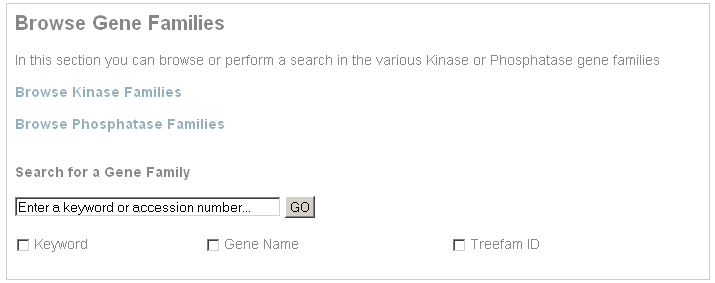
\includegraphics[scale=0.6]{pictures/BrowseGeneFamilies.png}
\caption{The Browse Gene Families Tool.}
\label{browsegenefamilies}
\end{figure}
The Gene Families tool allows the user to search for different kinase or phosphatase gene families and display the corresponding evolutionary tree of the proteins that comprise each family.
At the moment, the database includes data for about 121 gene families, 86 of which are kinase gene families and the remaining 35 are phosphatase gene families.
All this data has been obtained from the Treefam data source, which was described in more detail in a previous section.
Finally, this data involves only manually curated and not computer generated gene families.

The tool itself consists of two distinct components.
The first component provides two links which can be used in order to display all kinase gene families or all phosphatase gene families in the database.
Subsequently the user can click on the ``View Tree" link for the family he/she is interested in and the corresponding evolutionary tree provided by Treefam will be displayed on screen.
This tree has been pre-generated by the developers of Treefam and it is being accessed directly from their database.
The second component of the Gene Family tool is a search box where the user can enter a keyword and search for a gene family that is relevant to it.
Once the user clicks on the ``GO" button, a results page appears containing all gene families that contain the given keyword.
Finally the user can view the evolutionary tree of a gene family by clicking on the ``View Tree" link as explained previously.
